\documentclass[tikz,border=3pt]{standalone}
\usetikzlibrary{calc}
\usetikzlibrary{intersections,through}

\begin{document}
    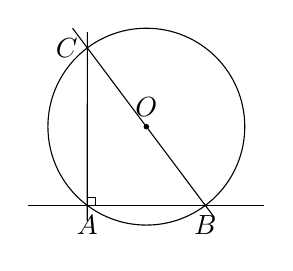
\begin{tikzpicture}[]
        % 标记两点, 做直线
        \coordinate (M) at (-.5,0);
        \coordinate (N) at (2.5,0);
        \draw [name path=l] (M) -- (N);
        % 标记圆心并画圆
        \coordinate [label=$O$] (O) at (1,1);
        \fill (O) circle(1pt);
        \coordinate (P) at ($(O)+(1.25,0)$);
        % 圆被标记为o
        \draw (O) circle (1.25);
        \coordinate [name path=o,circle through=(P)] (o) at (O);

        % 找交点并标记A,B
        \path [name intersections={of=l and o}] 
            coordinate [label=below:$A$] (A) at (intersection-1)
            coordinate [label=below:$B$] (B) at (intersection-2);
        % 绘制斜线
        \draw [name path=l2] ($(B)!-.15!(O)$) -- ($(B)!2.25!(O)$);
        % 标记C点: 圆与斜线的交点
        \path [name intersections={of=l2 and o}] 
            coordinate [label=left:$C$] (C) at (intersection-1);
        % 连接CA
        \draw ($(C)!-.1!(A)$) -- ($(C)!1.1!(A)$);
        % 标记直角
        \draw (A) rectangle ($(A)+(.1,.1)$);
    \end{tikzpicture}
\end{document}